%%%%%%%%%%%%%%%%%%%%%%%%%%%%%%%%%%%%%%%%%%%%%%%%%%%%%%%%%%%%%%%%%%%%%%%%%%%%
% AGUtmpl.tex: this template file is for articles formatted with LaTeX2e,
% Modified March 2013
%
% This template includes commands and instructions
% given in the order necessary to produce a final output that will
% satisfy AGU requirements.
%
% PLEASE DO NOT USE YOUR OWN MACROS
% DO NOT USE \newcommand, \renewcommand, or \def.
%
% FOR FIGURES, DO NOT USE \psfrag or \subfigure.
%
%%%%%%%%%%%%%%%%%%%%%%%%%%%%%%%%%%%%%%%%%%%%%%%%%%%%%%%%%%%%%%%%%%%%%%%%%%%%
%
% All questions should be e-mailed to latex@agu.org.
%
%%%%%%%%%%%%%%%%%%%%%%%%%%%%%%%%%%%%%%%%%%%%%%%%%%%%%%%%%%%%%%%%%%%%%%%%%%%%
%
% Step 1: Set the \documentclass
%
% There are two options for article format: two column (default)
% and draft.
%
% PLEASE USE THE DRAFT OPTION TO SUBMIT YOUR PAPERS.
% The draft option produces double spaced output.
%
% Choose the journal abbreviation for the journal you are
% submitting to:

% jgrga JOURNAL OF GEOPHYSICAL RESEARCH
% gbc   GLOBAL BIOCHEMICAL CYCLES
% grl   GEOPHYSICAL RESEARCH LETTERS
% pal   PALEOCEANOGRAPHY
% ras   RADIO SCIENCE
% rog   REVIEWS OF GEOPHYSICS
% tec   TECTONICS
% wrr   WATER RESOURCES RESEARCH
% gc    GEOCHEMISTRY, GEOPHYSICS, GEOSYSTEMS
% sw    SPACE WEATHER
% ms    JAMES
% ef    EARTH'S FUTURE
%
%
%
% (If you are submitting to a journal other than jgrga,
% substitute the initials of the journal for "jgrga" below.)

\documentclass[draft,gc]{AGUTeX}
% To create numbered lines:

% If you don't already have lineno.sty, you can download it from
% http://www.ctan.org/tex-archive/macros/latex/contrib/ednotes/
% (or search the internet for lineno.sty ctan), available at TeX Archive Network (CTAN).
% Take care that you always use the latest version.

% To activate the commands, uncomment \usepackage{lineno}
% and \linenumbers*[1]command, below:
%\usepackage{natbib} 
\usepackage{lineno}
\usepackage{textcomp}
\linenumbers*[1]

%  To add line numbers to lines with equations:
%  \begin{linenomath*}
%  \begin{equation}
%  \end{equation}
%  \end{linenomath*}
%%%%%%%%%%%%%%%%%%%%%%%%%%%%%%%%%%%%%%%%%%%%%%%%%%%%%%%%%%%%%%%%%%%%%%%%%
% Figures and Tables
%
%
% DO NOT USE \psfrag or \subfigure commands.
%
%  Figures and tables should be placed AT THE END OF THE ARTICLE,
%  after the references.
%
%  Uncomment the following command to include .eps files
%  (comment out this line for draft format):
\usepackage{graphicx}

%
%  Uncomment the following command to allow illustrations to print
%   when using Draft:
\setkeys{Gin}{draft=false}
%
% Substitute one of the following for [dvips] above
% if you are using a different driver program and want to
% proof your illustrations on your machine:
%
% [xdvi], [dvipdf], [dvipsone], [dviwindo], [emtex], [dviwin],
% [pctexps],  [pctexwin],  [pctexhp],  [pctex32], [truetex], [tcidvi],
% [oztex], [textures]
%
% See how to enter figures and tables at the end of the article, after
% references.
%
%% ------------------------------------------------------------------------ %%
%
%  ENTER PREAMBLE
%
%% ------------------------------------------------------------------------ %%

% Author names in capital letters:
\authorrunninghead{FEINBERG ET AL.}

% Shorter version of title entered in capital letters:
\titlerunninghead{THREE-AXIS LOW-TEMPERATURE REMANENCE}

%Corresponding author mailing address and e-mail address:
%\authoraddr{Corresponding author: J.M. Feinberg,
%Institute for Rock Magnetism, Department of Earth Sciences,
%University of Minnesota, MN 55455, USA.
%(feinberg@umn.edu)}

\begin{document}

%% ------------------------------------------------------------------------ %%
%
%  TITLE
%
%% ------------------------------------------------------------------------ %%


\title{Full vector low-temperature magnetic measurements of geologic materials}

%% ------------------------------------------------------------------------ %%
%
%  AUTHORS AND AFFILIATIONS
%
%% ------------------------------------------------------------------------ %%


%Use \author{\altaffilmark{}} and \altaffiltext{}

% \altaffilmark will produce footnote;
% matching \altaffiltext will appear at bottom of page.

\authors{Joshua M. Feinberg\altaffilmark{1}, Peter A. Solheid\altaffilmark{1},  Nicholas L. Swanson-Hysell\altaffilmark{1,2}, Mike J. Jackson\altaffilmark{1}, and Julie A. Bowles\altaffilmark{1,3}}% * <peat@umn.edu> 2014-09-19T14:51:09.726Z:
%
% Why doen't mike get a middle initial?
%
% ^ <feinberg@umn.edu> 2014-09-19T20:09:08.356Z.

\altaffiltext{1}{Institute for Rock Magnetism, Department of Earth Sciences, University of Minnesota, Minneapolis, Minnesota, USA}

\altaffiltext{2}{Department of Earth and Planetary Science, University of California, Berkeley, California, USA}

\altaffiltext{3}{Department of Geosciences, University of Wisconsin, Milwaukee, WI, USA}

%% ------------------------------------------------------------------------ %%
%
%  ABSTRACT
%
%% ------------------------------------------------------------------------ %%

% >> Do NOT include any \begin...\end commands within
% >> the body of the abstract.

\begin{abstract}
The magnetic properties of geologic materials offer insights into an enormous range of important geophysical phenomena ranging from inner core dynamics to paleoclimate. Often it is the low-temperature behavior ($<$300 K) of magnetic minerals that provides the most useful and highest sensitivity information for a given problem. Conventional measurements of low-temperature remanence are typically conducted on instruments that are limited to measuring one Cartesian component of the magnetization vector and are optimized for measurements in strong fields. These instrumental limitations have prevented fully optimized applications and have motivated the development of a low-temperature probe that can be used for low-temperature remanence measurements along three axes using a standard 2G Enterprises SQuID rock magnetometer. In this contribution, we describe the design and implementation of this instrument and present data from five case studies that demonstrate the probe's considerable potential for future research: a polycrystalline hematite sample, a polycrystalline hematite and magnetite mixture, a single crystal of magnetite, a single crystal of pyrrhotite and samples of  Umkondo Large Igneous Province diabase sills.
\end{abstract}

%% ------------------------------------------------------------------------ %%
%
%  BEGIN ARTICLE
%
%% ------------------------------------------------------------------------ %%

% The body of the article must start with a \begin{article} command
%
% \end{article} must follow the references section, before the figures
%  and tables.

\begin{article}

%% ------------------------------------------------------------------------ %%
%
%  TEXT
%
%% ------------------------------------------------------------------------ %%

\section{Introduction}

Magnetic behavior at low temperatures ($<$300 K) is one of the most sensitive indicators of the iron mineral phases and their  concentrations and grain size distributions in natural samples. Changes in magnetocrystalline anisotropy and crystallographic structure give rise to low-temperature transitions that are diagnostic of specific mineral phases. The Morin transition of hematite (at $\sim$262 K; \cite{Morin1950a}), the Verwey transition of magnetite (at $\sim$122 K; \cite{Verwey1939a}) and the Besnus transition of pyrrhotite (at $\sim$32 K, \cite{Besnus1964a}) are all diagnostic of common magnetic minerals that carry remanence at Earth surface temperatures. Other phases that acquire remanence at low temperature, such as siderite (with a Ne\'el temperature of 38 K; \cite{Frederichs2003a}) and superparamagnetic grains \citep{Worm1999a}, can also be readily identified through their low-temperature behavior. In addition to the utility of low-temperature data as a diagnostic tool for magnetic mineral identification and characterization, irreversible changes in remanence that are associated with cycling to low temperatures are often used as a tool in paleomagnetic studies. Low-temperature steps in paleodirectional and paleointensity study are applied in some protocols with the goal of preferentially removing magnetic remanence held by multidomain grains and thereby isolating magnetizations held by single-domain grains [e.g., \cite{Dunlop2003a, Yamamoto2003a}].

Low-temperature remanence experiments are routinely conducted on the Quantum Designs Magnetic Properties Measurement System (MPMS), most often with the intention of revealing information about the dominant magnetic mineral phases and grain size distribution. While these instruments are adept at a range of low-temperature experiments, understanding the full behavior of a rock's natural remanence at low-temperature is hampered by the measurement capabilities being limited to a single axis and the instrument not providing an ultra-low field environment. If low-temperature measurements of a natural remanence (NRM) are desired using such instrumentation, great care must be taken to align the NRM with the measurement axis, and any directional change during thermal cycling will not be captured. In such an instrument, deviation from the single-axis in such a system will result in a measured magnetization that is less than the specimen's actual total magnetization.

In this contribution, we describe a low-temperature probe developed for use with superconducting rock magnetometers (SRM) at the Institute for Rock Magnetism (\textit{IRM}), University of Minnesota. This instrument allows for three-axis measurements of magnetic remanence at temperatures between 300 and 17 K in low-field environments ($<$10 nT). It was developed with different engineering, but the same intent, as a low-temperature insert that has previously been implemented at the University of Rochester Paleomagnetic Laboratory \citep{Smirnov2011a}.

\section{Instrument design}

In order to develop the capacity to make three-axis measurements of remanence in a ultra-low-field environment, a cryostat insert was developed at the \textit{IRM} in cooperation with ColdEdge Technologies (Allentown, PA) (Figure \ref{fig:insert_schematic}). This low-temperature instrument (IRM-LTI) allows for three-axis measurements to be made between room temperature and $\sim$17 K using horizontal-loading SRMs. There are many advantages to outfitting a superconducting rock magnetometer for measurements at low-temperatures. First, these instruments are specifically designed for three-axis remanence measurements, and ambient fields are minimized using a superconducting lead shield. Nulling fields are applied by external coils while the shield cools to superconducting temperatures, ultimately trapping a $\sim$2-3 nT field along all three cardinal directions. Moreover modern SRM instruments utilize DC-SQUID sensors that offer greater sensitivity than existing low-temperature magnetometers and susceptometers that rely on RF-SQUID sensors. A room-temperature, open-ended bore is present in all 2G Enterprises magnetometers, allowing samples to be easily moved into and out of the measurement region of the instrument. 

The cryogenic insert is cooled by a pneumatically-driven SHI Displex SH-204 10K two-stage cryocooler with a 73.7-cm copper cold tip extension and 3.8-cm diameter stainless steel vacuum shroud (Figure \ref{fig:insert_schematic}). A 40.6-cm sapphire cold tip extension and sapphire radiation shield are joined to the end of the copper extension in order to prevent any radio frequency noise from traveling down the copper extension tip into the measurement region of the magnetometer. Sapphire at low temperatures has a high thermal conductivity, comparable to that of copper below 100K. A fiberglass vacuum shroud extension mounts to the stainless steel shroud to provide a non-metallic extension to the vacuum insulation space. Additional temperature control is provided by a non-inductively wound, 50-watt cartridge heater integrated into the body of the probe and mounted out of the sensor region, 40.6 cm away from the sample. The temperature inside the probe is monitored directly at the sample using a non-magnetic, fiber-optic temperature sensor (NeoOptics T1 probe) and two silicon diode sensors, one mounted on the copper cold tip extension near the heater and one mounted on the first stage of the cryocooler to monitor the radiation shield temperature. The probe assembly is mounted on a computer-controlled translation table driven by a stepper motor for automated movement in and out of the magnetometer, enabling background and sample measurements to be made throughout cooling/warming cycles.

Samples can be affixed to the end of the sapphire extension tip in a variety of ways. The goal is to maximize the thermal contact conductance between a sample and the sapphire extension tip. In its simplest form, samples can be affixed using Kapton tape, but at temperatures below $\sim$50 K, samples may lose efficient thermal contact with the sapphire extension tip.  Alternatively, a threaded copper sample holder can be bonded to the end of the sapphire extension tip, allowing samples to be held in thermal contact with the sapphire (Figure \ref{fig:insert_schematic}). Both of these methods allow for samples with maximum cylindrical dimensions of 9 mm diameter and 5 mm height.

Measurements without any sample show maximum magnetizations of ca. 3 x 10$^{-8}$ Am$^2$ with some degree of temperature dependence (see supporting information). The temperature-dependent magnetization of the LTI is largely repeatable, and empty probe experiments are conducted prior to measurement runs to enable background subtraction if deemed necessary. Samples can be cooled from room temperature to $\sim$17 K over the course of about three hours and then heated back to room temperature over another three to four hours. Thus, the time required to collect low temperature data using the IRM-LTI is roughly three times that required for the simplest low temperature experiments on the MPMS.  Alternatively, a user can define a more narrow temperature range for more detailed studies of low temperature phenomena.  

The approach and technical design of the LTI in this study (IRM-LTI) builds on ideas of an earlier effort by the late William Goree of 2G Enterprises along with Aleksey Smirnov and John Tarduno \citep{Smirnov2011a}. The key innovation of that collaborative effort was the design of a low-temperature instrument (that we will refer to as the ST-LTI) that could be inserted into a standard bore 2G Enterprises cryogenic rock magnetometer. In the ST-LTI, the sample was cooled by direct conduction in a bath of continually flowing liquid He. The sensors of the magnetometer were protected from the cooled low-temperature probe by a doubled-walled fiberglass tube, which was continually evacuated by a vacuum pump during measurements. Sample temperatures were monitored by a diode temperature sensor, which by necessity, was located about 10 cm behind the sample in order to avoid interference with the magnetometer pick-up coils. 

The design of the LTI in this study (IRM-LTI) has several advantages and disadvantages when compared to the ST-LTI. One comparative disadvantage of the IRM-LTI is that the volume of instrumental material introduced into the measurement region of the magnetometer is greater than that of the ST-LTI, and background signals are consequently larger.  The IRM-LTI is also intrinsically somewhat slower than the ST-LTI or the MPMS, since heat must be transported by solid-state conduction through a long rod rather than by advection in a fluid. Comparative advantages include: (1) because the IRM-LTI is moved via a translation table during measurements it is possible to quantify and adjust for background magnetization and magnetometer drift for each measurement; (2) this translation allows for the possibility of inline treatments, such as alternating-field demagnetization and acquisition of anhysteretic remanent magnetization and (3) utilizing a closed-cycle cryocooler systems allows the IRM-LTI to operate free of liquid helium. An additional positive aspect of the IRM-LTI is that it is currently available for community use through the Institute for Rock Magnetism's Visiting Fellowship Program (http://www.irm.umn.edu/IRM/applying.html).    

\section{Case studies using the instrument}
The five case studies that follow serve three primary purposes:
\begin{enumerate}
\item They aim to demonstrate that the temperature-dependent intensity data acquired using the IRM-LTI is virtually identical to that acquired using MPMS instruments (as shown by \cite{Smirnov2011a} for the ST-LTI), which should give confidence to potential users. 
\item They aim to demonstrate the utility of three-axis full-vector magnetic measurements in several different rock magnetic and paleomagnetic applications. In the course of doing so, novel results have been obtained.
\item It is hoped that these case studies will inspire new uses for the IRM-LTI, and in some instances we have provided suggestions for future studies that we have not yet explored. 
\end{enumerate}

\subsection{Polycrystalline Hematite}

A polycrystalline sample of hematite from Labrador, Canada with a strong foliation was pulsed in a 1.2 T field approximately perpendicular to the foliation plane to impart an isothermal remanent magnetization (IRM). Room temperature remanence in a single crystal of hematite falls within the basal plane, while remanence below the Morin transition is oriented along the normal to this plane. The strong shape-preferred alignment of the hematite grains in this polycrystalline sample allows us to explore whether its remanence direction shifts after cooling through the Morin transition. After being imparted, the IRM was cycled from room-temperature to $\sim$130 K using the IRM-LTI in conjunction with an SRM (Figure \ref{fig:hematite}A). The specimen underwent a significant loss of remanence as it cooled through the Morin transition which is partially recovered as the sample warmed back through the transition temperature (Figure \ref{fig:hematite}A,C). During this low-temperature cycling, the sample's directional remanence remained subparallel to the foliation normal (i.e. on average approximately parallel to the c axes of the individual crystals) and did not migrate towards the plane of the magnetic fabric (Figure \ref{fig:hematite}B). Even without any background correction, the majority of the remanence lies close to the z-axis of the stereonet. However, there is a 15-degree deflection in inclination away from 90 degrees (Figure \ref{fig:hematite}B). This deflection can be attributed to the magnetization of the IRM-LTI itself. The IRM-LTI's magnetization and low-temperature behavior can be important when measuring low remanence samples and background subtraction is necessary. This particular experiment was conducted when the IRM-LTI was outfitted with a relatively magnetic silicon diode thermometer that contributed to a background signal of $\sim$10$^{-6}$ Am$^2$. Subsequent improvements to the instrumental set-up have led to the current use of a far less magnetic fiber-optic temperature sensor that contributes $\sim$10$^{-8}$ Am$^2$ to the background signal.  By measuring the low-temperature cycling of the IRM-LTI without a mounted sample, we can characterize the background of the instrument and then subtract this influence from the measured sample data. When this background subtraction is done for the hematite sample, the data are tightly grouped near 90 degrees of inclination, illustrating the uniformity of the magnetization in the direction of the applied IRM before and after cooling through the Morin transition (Figure \ref{fig:hematite}B). The fact that the remamence remains parallel to the original applied field direction thoughout the experiment suggests either that the alignment of the hematite crystals was not perfect (otherwise the remanence would have fallen within the basal plane) and/or that the remanence was held by defects within hematite.

In this instance, the data collected with the three-axis IRM-LTI are very similar to those collected with a 1-axis MPMS (Figure \ref{fig:hematite}C).  The ratio of the room temperature remanence before and after low temperature cycling is nearly identical. One subtle difference between the two data sets is the slightly lower estimates of the Morin transition temperature on cooling and warming from the IRM-LTI (257.4 K) as compared to the MPMS (259.4 K; see supporting online materials for details on these estimates of transition temperature).  One possible explanation for this minor difference is a small thermal lag within the IRM-LTI. Additional measurements at a variety of cooling rates will test this explanation in the future.    

\subsection{Mixed assemblage of hematite and magnetite}

A polycrystalline hematite specimen containing trace amounts of magnetite was imparted with a 1.2 T IRM along the X-axis of the specimen. Following this treatment, the specimen was cooled to $\sim$20 K and then warmed back to room temperature inside the probe (Figure \ref{fig:naco}). This measurement is roughly equivalent to the room-temperature saturation isothermal remanent magnetization (RT-SIRM) experiments routinely conducted on MPMS instruments, and allows one to explore how the remanence of each phase evolves during low temperature cycling from room temperature to 20 K. The effects of the Morin and Verwey transitions are quite prominent as the sample was cycled to and from low-temperature while the direction of the magnetization did not vary (Fig. \ref{fig:naco}A).

After completion of the IRM-LTI experiment, a 1.2-T IRM was applied along the specimen's Z-axis and thermally cycled using an MPMS. Comparison of the IRM-LTI and MPMS data shows the results to be quite similar (Fig. \ref{fig:naco}B). Two subtle differences can be seen between the two data sets: (1) there is a systematic $\sim$2 K shift of the Morin and Verwey transitions towards cooler temperatures in the IRM-LTI data compared to the MPMS data (see supporting online materials for details), as was seen with the Labrador hematite sample (Figure \ref{fig:hematite}C), and similar to the temperature offset observed by Smirnov and Tarduno in the ST-LTI experiments; (2) the magnitude of the magnetization is slightly less for the MPMS data than the total vector of the three-axis IRM-LTI data, suggesting that some of the magnetization may have been off-axis during the MPMS experiment and thereby not detected by the single-axis measurement capabilities of that instrument.

In future studies, the IRM-LTI can be used to disentangle the remanence held by each of these phases by imparting specimens with multiple, mutually perpendicular magnetizations, similar in style to a Lowrie test \citep{Lowrie1990a}, where the remanence associated with specific phases is forced to lie along different cardinal directions. In this way, the IRM-LTI may provide a unique method for non-destructive exploration of the temperature-dependent magnetic behavior of mixed magnetic mineral assemblages. 

\subsection{Single crystal of magnetite}

A square-based pyramid was cut from a magnetite octahedron to explore the directional behavior of remanence for a single crystal of multidomain magnetite during low temperature cycling using the IRM-LTI. The 2-mm subspecimen used in this study was prepared using a low-speed saw to remove the pyramid from the top of a natural magnetite octahedron that originated in the Central African Republic (mined and sold by IKON). Three experiments were conducted, each of which consisted of applying a strong (1.2 T) IRM in a distinct direction and then cycling that magnetization to low-temperature (20 K) and back. A schematic drawing of the specimen and its orientation relative to the measurement axes of the superconducting rock magnetometer (SRM) and to the orientations of three separate 1.2 T IRMs is shown in Figure \ref{fig:magnetite1}A. We attempted to impart these IRMs along the [-111], [100], and [0-1-1] of magnetite because these directions correspond to magnetocrystalline easy, hard, and intermediate axes, respectively, at room temperature. As magnetite cools below the Verwey transition (T$_{V}$), the mineral experiences a first-order phase transition where its crystal symmetry changes from cubic (c) to monoclinic (m). The orientations of the \textit{a}, \textit{b}, and \textit{c} axes of the resulting monoclinic magnetite will depend on the magnetic environment in which this transition occurs, but by convention are described as [001]$_{m}$//[001]$_{c}$. [100]$_{m}$//[110]$_{c}$, and [010]$_{m}$//[-110]$_{c}$. The easy, intermediate, and hard magnetocrystalline axes for monoclinic magnetite are [001]$_{m}$, [010]$_{m}$, and [100]$_{m}$, respectively. The low temperature cycling of the isothermal remanence applied to the specimen is described in detail below, but it is important to note that there are multiple sources of orientation error that are inherent to the measurements.  First, despite the care taken during specimen preparation, it is likely that the square base of the pyramid was not cut exactly parallel to the (100) of magnetite and may be misaligned by $<10^{\circ}$. Such an error will affect all of the directional IRM experiments.  Second, for each IRM there may be a small $<10^{\circ}$ error between the orientation of the applied field and its targeted crystallographic direction. Third, there is also a small ($<5^{\circ}$) error associated with placement of the specimen back on the end of the IRM-LTI after each successive IRM. This latter error should only be rotational around the Z-axis of the magnetometer.     

Figure \ref{fig:magnetite1}B shows the directional results of the low temperature cycling of the three separate IRMs. The alignment of the IRM remanence with the intended magnetocrystalline axes of the magnetite is broadly similar to the experimental scheme. There are no dramatic changes in remanence direction during low temperature cycling regardless of the orientation of the applied IRM. During cooling from room temperature the remanence of all three IRMs decreases towards the isotropic point (T$_{K}$ = 130 K) and Verwey transition (T$_{V}$ = 110 to 120 K), reaching a minimum at $\sim$118 K (Figure \ref{fig:magnetite1}C). The extent of this remanence drop is slightly directionally dependent: the percent loss in remanence from 260 K to the Verwey transition minima for the IRMs imparted along [-111], [100], and [0-1-1] are 68\%, 75\%, and 72\%, respectively. Thus, the remanence imparted along the cubic magnetocrystalline easy axis was marginally more resistant to low temperature demagnetization than those imparted along the intermediate or hard axes. On continued cooling through Tv, the remanence increases abruptly and significantly (Figure \ref{fig:magnetite1}C), unlike the behavior commonly observed for polycrystalline MD powder samples in MPMS experiments, but similar to that found in previous single-crystal measurements [e.g., \cite{Ozdemir1999a, Smirnov2011a}]. The magnitude of remanence below the Verwey transition is also somewhat anisotropic with the ratio of remanence at 20 K to that at 260 K for each IRM at 53\%, 61\%, and 56\%, respectively. Thus, remanence was more readily inherited by monoclinic magnetite when the original room-temperature IRM is applied parallel to its magnetocrystalline easy axis direction ([001]$_{m}$ or [001]$_{c}$). A third metric of anisotropy is seen after cycling back to 260 K, where the recovered remanence for the IRMs imparted along [-111], [100], and [0-1-1] is 44\%, 48\%, and 40\%, respectively. In this context, the most efficient remanence recovery occurred when the original IRM was imparted along the cubic magnetocrystalline hard axis. This persistent remanence is likely pinned by crystalline imperfections in the magnetite, such as dislocation networks (as recently imaged by \cite{Lindquist2014a}). The absolute value of the remanence on warming back to room temperature is nearly identical for all three IRM treatments (Figure \ref{fig:magnetite1}C), suggesting that regardless of the orientation of the initial IRM, after passing twice through T$_{V}$ and T$_{K}$ the final arrangement of domain walls in the specimen has achieved a common low-energy configuration. These results also show the incomplete nature of low-temperature demagnetization associated with MD-sized grains. However, as is shown in ARM data applied to an assemblage of MD magnetite in a coarse-grained diabase sample below, it is likely that the portion of magnetization that was demagnetized is the lowest coercivity fraction. In this case study, we examine a single, large MD grain and show that a minimum of a third of its remanence is routinely retained after low-temperature cycling. The low-temperature behavior of MD magnetite is further discussed below in section 3.5, and has important implications for paleomagnetic and paleointensity studies that use low-temperature demagnetization steps to minimize the unwanted contributions from MD grains. 

The data acquired by the IRM-LTI also allow users to see subtle, but important details that are often lost in one-axis MPMS measurements.  For example, the distinct magnetic behaviors as the magnetite passes through its Verwey transition near 118 K and its isotopic point near 130 K are well-resolved in the three-axis data (Fig. \ref{fig:magnetite2}). Another interesting observation from the three-axis data is the change in the remanence direction in series 2 (where the 1.2 T  IRM was applied approximately parallel to the [100] direction) wherein there is subtle clockwise movement on cooling that is reversible on warming.  There are two distinct clusters of directions: one cluster is defined by all data collected above 115 K, while the second cluster is comprised of all data collected below 115 K.  Measurements collected at 115 K on both cooling and warming are at an intermediate position (Figure \ref{fig:magnetite2}). The vector component diagram in Figure \ref{fig:magnetite2}C also shows this behavior along with the concomitant change in intensity before and after the Verwey transition. The crystallographic origins of this directional movement require further study, but one likely influence is the reorganization of ferroelastic twins as the sample is converted from one crystal system to the other [e.g., \cite{Kasama2010a}].         

\subsection{Single crystal of pyrrhotite}

A single crystal of pyrrhotite measuring $\sim$2.5 by $\sim$3.5 by $\sim$4.5 mm was used to explore the directional behavior of remanence for multidomain pyrrhotite during low-temperature cycling using the IRM-LTI. Pyrrhotite often occurs in nature as intergrowths of hexagonal and monoclinic iron sulfide, the latter of which is ferrimagnetic at room temperature. Monoclinic pyrrhotite experiences a dramatic change in its magnetic properties at $\sim$35 K (\cite{Besnus1964a}); the underlying crystallographic and/or magnetocrystalline changes are still debated \citep{Wolfers2011a, Kind2013a}. The details of the mineral's crystal symmetry and internal microstructures are highly complex owing to nonstoichiometry in the Fe$_{1-x}$S system and non-regular ordering of vacancies within the crystal lattice.  Crystallographers frequently take a simplified view of the mineral in referring to its crystal symmetry as `pseudohexagonal.' Above the Besnus transition, pyrrhotite exhibits a `hard' magnetic axis along the c direction and remanence tends to lie within the basal plane defined by the a$_{1}$, a$_{2}$, and a$_{3}$ axes. A secondary electron micrograph of the single-crystal specimen used in this study is shown in Figure \ref{fig:pyrrhotite}A (collected with a JEOL 6500 FEG-SEM operated at 20 kV with a working distance of 22.8 mm). The orientations of the crystal's pseudohexagonal crystallographic axes were measured using electron backscatter diffraction (EBSD) and are shown in Figure \ref{fig:pyrrhotite}A. Prior to measurement in the IRM-LTI, the sample was oriented such that the a$_{1}$ axis was subparallel to the X-axis of the magnetometer.  The remanence of the sample was noted and then the threaded copper sample holder was tightened onto the sample mounting surface to ensure thermal contact, resulting in a counter-clockwise rotation of the a$_{1}$ axis of 10$^{\circ}$ to 30$^{\circ}$. IRMs were imparted to the sample in a number of orientations prior to low temperature cycling in the IRM-LTI, and the intended directions are shown as blue points in the equal area plots in Figure \ref{fig:pyrrhotite}C. As was the case with the single-crystal magnetite measurements, there are likely small angular errors between the actual and intended applied field directions for IRM acquisition.  

Figure \ref{fig:pyrrhotite}C shows the directions throughout low-temperature demagnetization of three separate 1.2-T IRMs imparted along different crystallographic directions. The leftmost equal area plot in Figure \ref{fig:pyrrhotite}C shows the low-temperature demagnetization of an IRM imparted along an angle bisecting the pyrrhotite a$_{1}$ and c axes. The resulting remanence falls almost directly along the a$_{1}$ axis Figure \ref{fig:pyrrhotite}C. This difference in applied field direction and the acquired remanence is likely due to the strong anisotropy given that remanence in pyrrhotite prefers to lie within the basal plane of the pseudohexagonal structure. During cooling and warming the remanence direction remains largely unchanged, but does track slightly along a great circle that includes the c-axis. After passing through the Besnus transition on cooling the remanence at 20 K is only 10\% of the value at 290 K. After warming back to 290 K, the final residual remanence is 18\% of the original remanence at 290 K (see supporting online materials).

The middle equal area plot in Figure \ref{fig:pyrrhotite}C shows an IRM imparted along the c-axis. The resulting remanence falls along the -a$_{1}$ direction, again indicating the strong tendency at room temperature for remanence in pyrrhotite to lie within the basal plane. As in the case for the low-temperature cycling the IRM that bisected c and a$_{1}$, the remanence direction remained relatively stable during low temperature cycling. However, after passing through the Besnus transition on cooling the remanence of this IRM at 20 K is 25\% of the value at 290 K. After warming back to 290 K, the final residual remanence is 17\% of the original remanence at 290 K (Figure \ref{fig:pyrrhotite}B). Although there is something about an IRM applied along the pyrrhotite c-axis that allows for a greater percentage of its remanence to be retained after cooling through the Besnus transition, the final percentage of residual remanence after warming back to room temperature consistently appears to be $\sim$17\%.    

The rightmost equal area plot in Figure \ref{fig:pyrrhotite}C shows an IRM imparted along an angle that bisects the a$_{1}$ and -a$_{3}$ directions. In this instance the resulting remanence direction appears to be oriented roughly parallel to the applied field direction, suggesting that pyrrhotite remanence is not constrained to lie solely along the a$_{i}$ axes, but may be oriented suparallel to the applied field within the basal plane. After passing through the Besnus transition on cooling the remanence at 20 K is 18\% of the value at 290 K. After warming back to 290 K, the final residual remanence is 22\% of the original remanence at 290 K. Thus, a higher percentage of remanence seems to be retained after cycling through the Besnus transition if an IRM is applied along a direction within the basal plane. 

\subsection{Samples from the interior of Umkondo large igneous province sills}

Many rocks carry complex multicomponent natural remanent magnetizations, with different generations of magnetization acquired at different times by separate mechanisms and carried in varying proportions by different populations of magnetic grains. For such heterogeneous magnetizations, significant directional changes may accompany passage through transitions and isotropic points as different components are affected according to the mineralogy, defect structures, and grain sizes of their carriers. Just as continuous high-temperature thermal demagnetization can provide crucial observations for correctly interpreting a sample's remanence \citep{Wack2007a, Coe2014a}, full-vector measurements during low-temperature cycling of such samples may also provide a new means of disentangling a rock's complex magnetization history. 

Bulk rock samples containing large populations of randomly-oriented magnetic crystals carrying a univectorial remanence (i.e., a magnetization acquired through a single process, in a relatively constant field orientation), are not expected to show large directional changes while passing through magnetic transitions. In such a scenario, the directional changes associated with the individual crystals should average out, and only a change in the magnitude of the remanence should be observed. This is the case for specimen PW15-4d, a coarse-grained diabase sill from the $\sim$1.1 Ga Umkondo Province of Botswana \citep{Hanson2004a}. Room-temperature alternating-field demagnetization experiments show that the NRM decays in a univectorial manner (Figure \ref{fig:Umkondo_PW15NRM}A). Traditional low-temperature demagnetization experiments involving submersion in a liquid N$_{2}$ bath result in a 52\% loss in NRM intensity (Figure \ref{fig:Umkondo_PW15NRM}A), suggesting that a significant fraction of the remanence is held by multidomain grains. Low-temperature cycling of the NRM in the IRM-LTI on a sister specimen from the same core shows that the remanence direction remains stationary while the intensity decreases significantly such that it is only 21\% of the initial NRM after cooling through the Verwey transition. The magnetization recovers to 52\% of the original NRM value upon warming back to room temperature (Figure \ref{fig:Umkondo_PW15NRM}B) resulting in a similar overall remanence loss as the liquid nitrogen bath on the sister specimen.

In order to explore whether low-coercivity magnetite loses its remanence at similar temperatures to higher-coercivity magnetite, this same specimen was given two mutually perpendicular anhysteretic remanent magnetizations (ARMs; Figure \ref{fig:Umkondo_ARM}). First, the specimen was given an ARM along its negative Z-axis (200 mT AF with a 100 $\mu$T DC bias field).  Then the specimen was imparted with a second more weakly held ARM along its negative x-axis (5 mT AF with a 200 $\mu$T DC bias field).  This second ARM targeted only those grains in the sample with coercivities $\leq$5 mT, and hence is a partial ARM (pARM). In contrast, the first ARM applied along the z-axisis held by higher coercivity grains ranging between 5 and 200 mT (referred to as 'ARM$_{Z}$' henceforth). On thermal cycling in the IRM-LTI, the remanence associated with ARM$_{Z}$ behaves in a manner similar to what is commonly observed in single-axis MPMS measurements, where remanence begins to decrease at $\sim$225 K and then decreases at an accelerating rate as it approaches T$_{V}$ (Figure \ref{fig:Umkondo_ARM}A). This pattern of remanence loss parallels the changes in the dominant magnetocrystalline energy term for cubic magnetite (K$_{1}$)(Figure \ref{fig:Umkondo_ARM}C). The isotropic point for magnetite, T$_{K}$, occurs near 130 K when K$_{1}$ changes from negative to positive. Thus, this pattern of remanence loss in magnetite during cooling is actually a two-stage process involving passage through both T$_{K}$ and T$_{V}$. During warming, the remanence associated with the ARM$_{Z}$ recovers to 71\% of its original value. This low-temperature memory is significant and is typical for single-domain and pseudo-single-domain grains, which are able to preserve their original remanence owing to shape anisotropy and pinned domain walls \citep{Dunlop1997a}. It is also likely that some of this remanence is held by multidomain grains with regions of high defect density that produce pinning coercivities higher than 5 mT.

By contrast, the pattern of remanence loss associated with the lower coercivity pARM is significantly different from that of the ARM$_{Z}$ (Figure \ref{fig:Umkondo_ARM}A,B). The lower coercivity remanence experiences a linear decrease from room temperature to T$_{V}$ that is seemingly unaffected by the rate of change in the K$_{1}$ magnetocrystalline energy term (Figure \ref{fig:Umkondo_ARM}C). This style of low temperature demagnetization behavior is novel and to our knowledge has not been observed in earlier studies of magnetite-bearing rocks, although \cite{Muxworthy2003a} did observe systematic changes in the shapes of M(T) cooling curves for pARMs acquired over different coercivity windows, in magnetites of differing grain sizes. Importantly, this behavior would be undetected in a conventional MPMS RT-SIRM measurement. There is no recovery of this remanence during warming back to room temperature (Figure \ref{fig:Umkondo_ARM}), suggesting that this remanence was held by multidomain grains whose domain wall configurations were dramatically rearranged during cycling through both T$_{K}$ and T$_{V}$. The final reamence direction following low-temperature cycling of the ARM$_{Z}$ + pARM$_{X}$ is very similar to the ARM$_{Z}$ direction prior to imparting pARM$_{X}$. This result demonstrates  the effectiveness of low-temperature demagnetization for the removal of remanence held by low-coercivity grains.

Some of the specimens from the Umkondo province sills show significant directional changes after thermal cycling in liquid N$_{2}$. Figure \ref{fig:Umkondo_PW10NRM} shows one such specimen, PW10-7a, whose NRM direction shifted by 64\textdegree after the low-temperature demagnetization (LTD) step. A conventional MPMS RT-SIRM measurement (see supporting online materials),  shows that 67\% of the room temperature remanence is lost through low-temperature demagnetization. However, the IRM-LTI provides a more complete picture, capturing this same broad behavior, but also documenting the progressive directional change throughout the experiment (Fig. \ref{fig:Umkondo_PW10NRM}). After passing through T$_{V}$, the remanence direction remains relatively constant during cooling to 20 K and subsequent rewarming to T$_{V}$. However, during warming from T$_{V}$ to room temperature the specimen's remanence direction shifts dramatically towards expected Umkondo orientations as the low temperature memory held by SD and PSD grains is preferentially recovered over magnetization held by MD grains that is not recovered. As a result, the overprint, secondary to the primary thermal remanent magnetization is largely, although not entirely, removed. These three-axis data demonstrate the effectiveness of low-temperature cycling as a tool for demagnetization of remanence held by MD grains. Furthermore, these data give a glimpse into the ''black box'' of progressive remanence change that occurs during routine liquid N$_2$ demagnetization of paleomagnetic samples.

\section{Future directions}

This study presents several examples demonstrating the utility of low-temperature remanence cycling using the IRM-LTI, but there are a multitude of additional research directions that can be explored using this instrument. From an experimental perspective, one of the more exciting applications for the IRM-LTI is the potential for in-line treatments at low temperatures. Examples include alternating field demagnetization and acquisition of anhysteretic remanence magnetization (ARM) or IRM. Such treatments would allow researchers to explore changes in the coercivity distributions of samples above and below important mineral transitions, such as the Morin, Verwey, and Besnus transitions. For nanoparticle populations, the joint distribution of grain size and microcoercivity f(\textit{V},\textit{H}$_{k0}$) can be obtained by AF demagnetization of weak-field TRMs at a set of low temperatures [c.f., \cite{Dunlop1969a}].  To enable such new experimental capabilities, the construction of in-line coils is currently underway at the \textit{IRM}. Additionally, as alluded to in Section 3.2, the IRM-LTI also has the potential to run three-axis Lowrie style thermal cycling experiments that can enable users to unmix the low-temperature remanence held by populations of different phases and grain sizes with greater confidence than possible with a single-axis instruments. This approach will provide information analogous to that obtained in traditional Lowrie tests, but without the potential for mineral alteration typically associated with thermal demagnetization experiments above room temperature.

The experimental flexibility of the IRM-LTI may make it possible to address many of the questions regarding fundamental magnetic behavior in important minerals such as magnetite, maghemite, titanomagnetite, hematite, griegite, and pyrrhotite. The IRM-LTI allows researchers to observe full-vector remanence changes as minerals pass through isotropic points, ordering temperatures, and blocking and unblocking temperatures. Processes such as TRM acquisition can be explored by measuring the remanence acquired by populations of superparamagnetic grains. Similarly, the effects of cooling rate on the intensity of remanence can be directly observed by modifying the rate at which specimens are cooled. By preparing specimens with varying degrees of mineral alignment it may also be possible to quantify the anisotropy of remanence. This is by no means an exhaustive exposition of the possible rock magnetic applications, but we hope that it illustrates the research potential of the instrument.     

The IRM-LTI can also provide complementary information to planetary scientists trying to isolate the primary magnetization of meteorites in order to learn more about the conditions that existed during the early history of the solar system. The assemblage of magnetic minerals found within meteorite samples is frequently far more complex than that found in terrestrial samples. Alloys of Fe, Ni, and S are common, as are varying concentrations of magnetite and titanomagnetite. The effects of shock on remanent magnetization further compound the difficulties of interpreting a meteorite’s complex thermomagnetic history. One process that has not received as much attention is the effect of low temperature thermal cycling on the remanent magnetism of the constituent magnetic minerals. The orbits of most asteroids and comets are eccentric, which guarantees that these objects will experience heating and cooling cycles during the course of their orbit around the Sun. Another process that may affect the magnetization of meteorites is “inverse” thermoremanent magnetization, which is acquired as magnetite is warmed through the Verwey transition or isotropic point \citep{Dunlop2006a}. This type of remanence could be acquired in Earth's field as meteorites warm to Earth surface temperatures and could contaminate paleointensity measurements. The IRM-LTI's low-temperature, three-component system allows researchers to design experiments to observe remanence changes that could result from thermal perturbations experienced by meteorites as they pass by the Sun (at solar perigee) or as they enter Earth’s atmosphere.

These applications form the basis for decades of potential future research; much more than could ever be accomplished by the authors of this study. The instrument was designed with a philosophy of making it affordable to other research groups and to be broadly compatible with horizontal-loading 2G Enterprises cryogenic magnetometers that are used in the majority of paleomagnetic laboratories. The IRM-LTI is currently housed at the Institute for Rock Magnetism at the University of Minnesota, where it is available to the international scientific community through the lab's NSF Visiting Fellowship program (http://www.irm.umn.edu/IRM/categories.html). It is hoped that this study will inspire colleagues to visit the IRM in order to the instrument to advance their own research programs.    

%%% End of body of article:

%%%%%%%%%%%%%%%%%%%%%%%%%%%%%%%%
%% Optional Appendix goes here
%
% \appendix resets counters and redefines section heads
% but doesn't print anything.
% After typing \appendix
%
%\section{Here Is Appendix Title}
% will show
% Appendix A: Here Is Appendix Title
%
%%%%%%%%%%%%%%%%%%%%%%%%%%%%%%%%%%%%%%%%%%%%%%%%%%%%%%%%%%%%%%%%
%
% Optional Glossary or Notation section, goes here
%
%%%%%%%%%%%%%%
% Glossary is only allowed in Reviews of Geophysics
% \section*{Glossary}
% \paragraph{Term}
% Term Definition here
%
%%%%%%%%%%%%%%
% Notation -- End each entry with a period.
% \begin{notation}
% Term & definition.\\
% Second term & second definition.\\
% \end{notation}
%%%%%%%%%%%%%%%%%%%%%%%%%%%%%%%%%%%%%%%%%%%%%%%%%%%%%%%%%%%%%%%%
%
%  ACKNOWLEDGMENTS

\begin{acknowledgments}

Bill Goree's career of developing and commercializing superconducting rock magnetometers for paleo- and rock magnetism continues to leave a substantial impact on our discipline. This project builds on his vision of a low-temperature insert that just before his passing in 2007 he envisioned would be best implemented with a liquid-free cyrocooler system. John Tarduno encouraged the development of this type of insert and provided valuable input based on his lab's experience with their flow-through system. We thank Aleksey Smirnov for providing the polycrystalline Labrador hematite sample. Richard Hanson played an important role in the field expedition during which samples were collected from Umkondo Sills. Functions from the open source PmagPy project (https://github.com/ltauxe/PmagPy) were used extensively for data plotting and we are grateful to the project's lead developer Lisa Tauxe. This research was funded by EAR-0929807 to J.M.F., EAR-1045635 to N.L.S.-H., and by support of the IRM by the NSF/EAR Instruments and Facilities program. This is IRM contribution 1409.

\end{acknowledgments}

%% ------------------------------------------------------------------------ %%
%%  REFERENCE LIST AND TEXT CITATIONS
%
% Either type in your references using
% \begin{thebibliography}{}
% \bibitem{}
% Text
% \end{thebibliography}
%
% Or,
%
% If you use BiBTeX for your references, please use the agufull08.bst file (available at % ftp://ftp.agu.org/journals/latex/journals/Manuscript-Preparation/) to produce your .bbl
% file and copy the contents into your paper here.
%
% Follow these steps:
% 1. Run LaTeX on your LaTeX file.
%
% 2. Make sure the bibliography style appears as \bibliographystyle{agufull08}. Run BiBTeX on your LaTeX
% file.
%
% 3. Open the new .bbl file containing the reference list and
%   copy all the contents into your LaTeX file here.
%
% 4. Comment out the old \bibliographystyle and \bibliography commands.
%
% 5. Run LaTeX on your new file before submitting.
%
% AGU does not want a .bib or a .bbl file. Please copy in the contents of your .bbl file here.

\bibliographystyle{agufull08}
\small\bibliography{NSH_allrefs}

%Reference citation examples:

%...as shown by \textit{Kilby} [2008].
%...as shown by {\textit  {Lewin}} [1976], {\textit  {Carson}} [1986], {\textit  {Bartholdy and Billi}} [2002], and {\textit  {Rinaldi}} [2003].
%...has been shown [\textit{Kilby et al.}, 2008].
%...has been shown [{\textit  {Lewin}}, 1976; {\textit  {Carson}}, 1986; {\textit  {Bartholdy and Billi}}, 2002; {\textit  {Rinaldi}}, 2003].
%...has been shown [e.g., {\textit  {Lewin}}, 1976; {\textit  {Carson}}, 1986; {\textit  {Bartholdy and Billi}}, 2002; {\textit  {Rinaldi}}, 2003].

%...as shown by \citet{jskilby}.
%...as shown by \citet{lewin76}, \citet{carson86}, \citet{bartoldy02}, and \citet{rinaldi03}.
%...has been shown \citep{jskilbye}.
%...has been shown \citep{lewin76,carson86,bartoldy02,rinaldi03}.
%...has been shown \citep [e.g.,][]{lewin76,carson86,bartoldy02,rinaldi03}.
%
% Please use ONLY \citet and \citep for reference citations.
% DO NOT use other cite commands (e.g., \cite, \citeyear, \nocite, \citealp, etc.).

%% ------------------------------------------------------------------------ %%
%
%  END ARTICLE
%
%% ------------------------------------------------------------------------ %%
\end{article}
%
%
%% Enter Figures and Tables here:
%
% DO NOT USE \psfrag or \subfigure commands.
%
% Figure captions go below the figure.
% Table titles go above tables; all other caption information
%  should be placed in footnotes below the table.
%
%----------------
% EXAMPLE FIGURE
%


\begin{figure}
\noindent\includegraphics[width=0.8\textwidth]{LowT_insert.pdf}
\caption{Components of the Institute for Rock Magnetism's low temperature instrument (IRM-LTI). The length of the instrument is 175 cm from the back of the cryocooler to the tip of the fiberglass vacuum shroud.}
\label{fig:insert_schematic}
\end{figure}

\begin{figure}
\noindent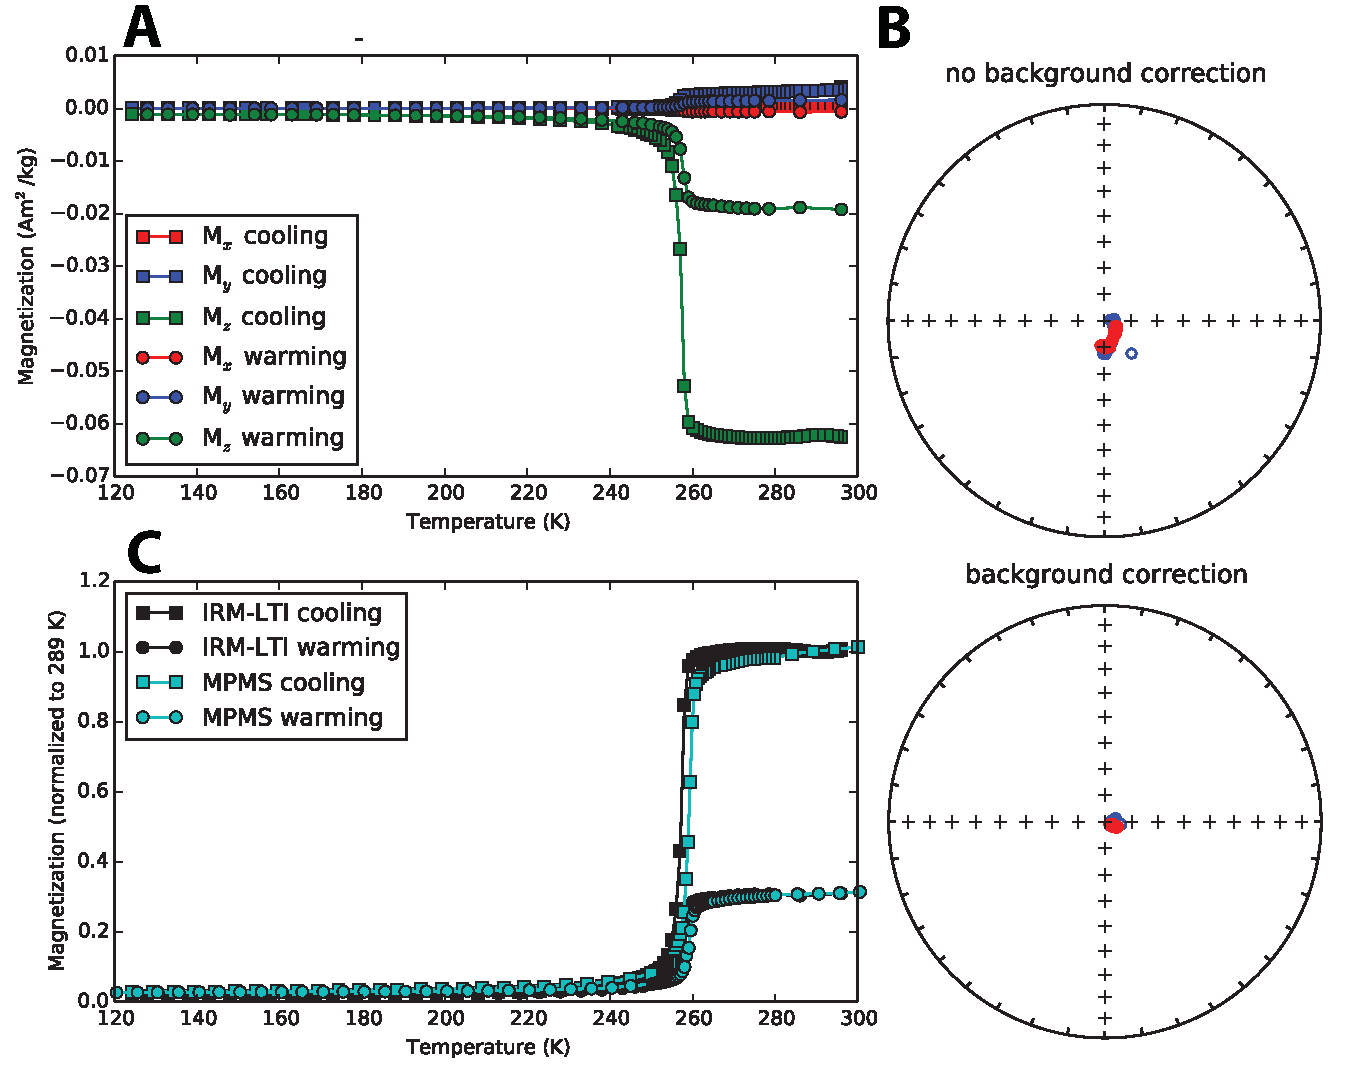
\includegraphics[width=\textwidth]{Hematite1.pdf}
\caption{Low temperature thermal cycling of IRMs for a sample of polycrystalline Labrador hematite. (a) Background-corrected three-axis remanence data for a 1.2 T IRM cycled to and from 120 K using the IRM-LTI. There is prominent remanence loss as the specimen cooled through the Morin transition ($\sim$258 K). (b) Equal area plots of the uncorrected and corrected directions throughout thermal cycling. Blue points are during cooling while red points are during warming. All data plot in the upper hemisphere. (c) Comparison between the total vector magnetization calculated from the three-axis IRM-LTI and 1-axis data collected for a similar experiment conducted on an MPMS.}
\label{fig:hematite}
\end{figure}

\begin{figure}
\noindent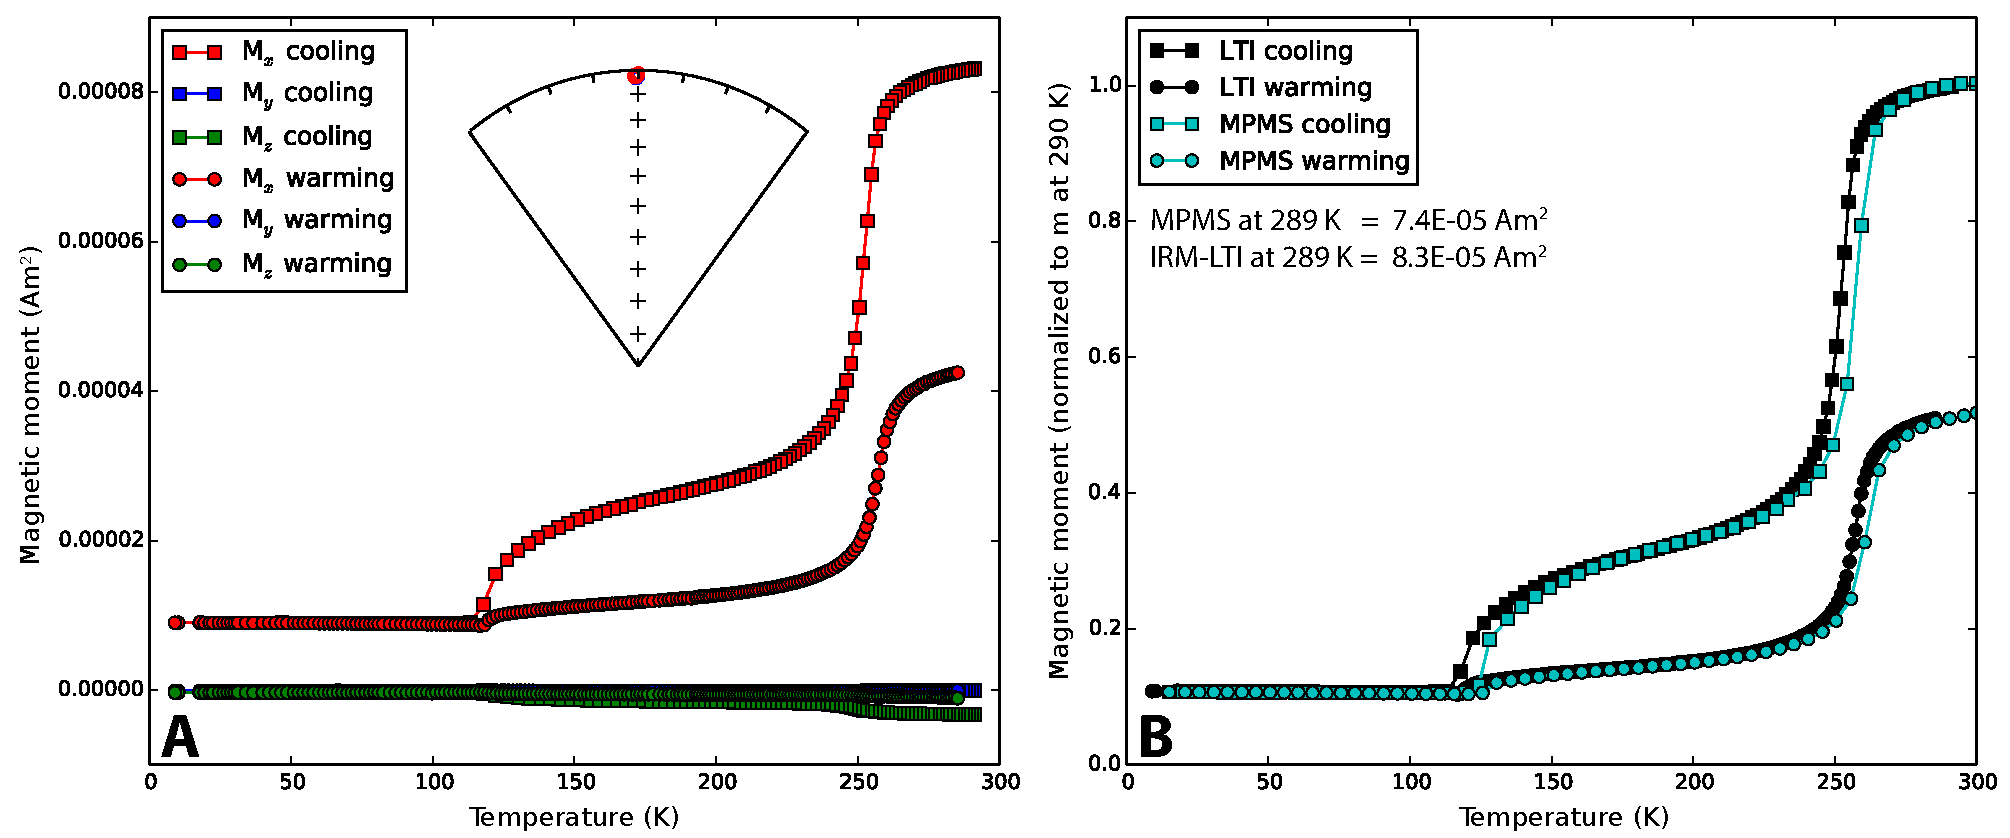
\includegraphics[width=\textwidth]{HemMag1.pdf}
\caption{Low temperature thermal cycling of a polycrystalline hematite sample containing trace quantities of magnetite. (a) plot of background-corrected, three-axis remanence data for cooling to 20 K and warming back to room temperature using the IRM-LTI following application of a 1.2-T isothermal remanence. Both the Morin and Verwey transitions are clearly resolved. The inset shows a portion of an equal area plot with the tightly grouped directions of all 114 data points measured during the thermal cycling. (b) plot of the total magnetization measured by the IRM-LTI and single-axis data obtained on an MPMS for a 1.2-T isothermal remanence as it was cycled to and from low temperature ($\sim$20 K). The data are normalized to the magnetization measured at $\sim$290 K on each respective instrument.}
\label{fig:naco}
\end{figure}

\begin{figure}
\noindent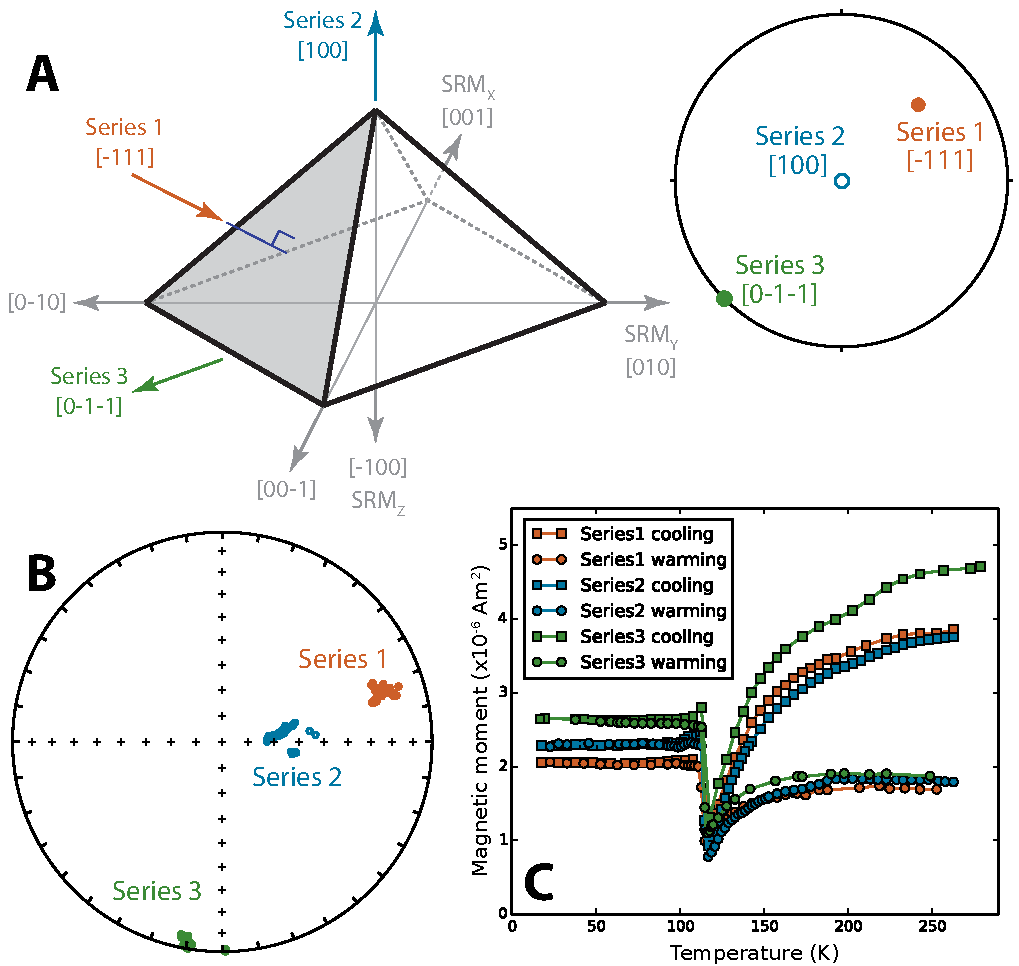
\includegraphics[width=\textwidth]{Magnetite1.pdf}
\caption{Low temperature thermal cycling of a specimen comprised of a single magnetite crystal. (a) schematic of the specimen depicting the orientation of the crystal axes along with the directions of the isothermal pulse magnetizations applied during the three experiments. (b) equal area plot of the directional data from each experiment. (c) full vector magnetization intensity for each of the three experiments during cooling (squares) and warming (circles).}
\label{fig:magnetite1}
\end{figure}

\begin{figure}
\noindent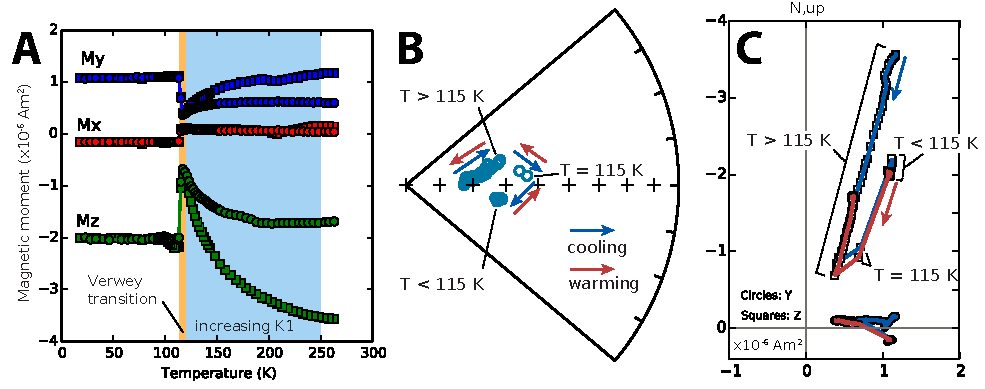
\includegraphics[width=\textwidth]{Magnetite2.pdf}
\caption{Data from the series 2 experiment (1.2 T IRM applied approximately along the [100] axis) on the single magnetite crystal. (a) three-axis remanence data for cooling to 20 K and warming back to room temperature using the IRM-LTI. (b) portion of an equal area plot of the remanence direction during thermal cycling illustrating the clockwise change that occurs as the sample is cooled through the Verwey transition. This directional change is reversible on warming. (c) vector component diagram where both the change in direction and increase in intensity can be seen across the Verwey transition. The blue line connects data points measured during the cooling portion of the experiment while the red line connects data points for the warming portion of the experiment.
}
\label{fig:magnetite2}
\end{figure}

\begin{figure}
\noindent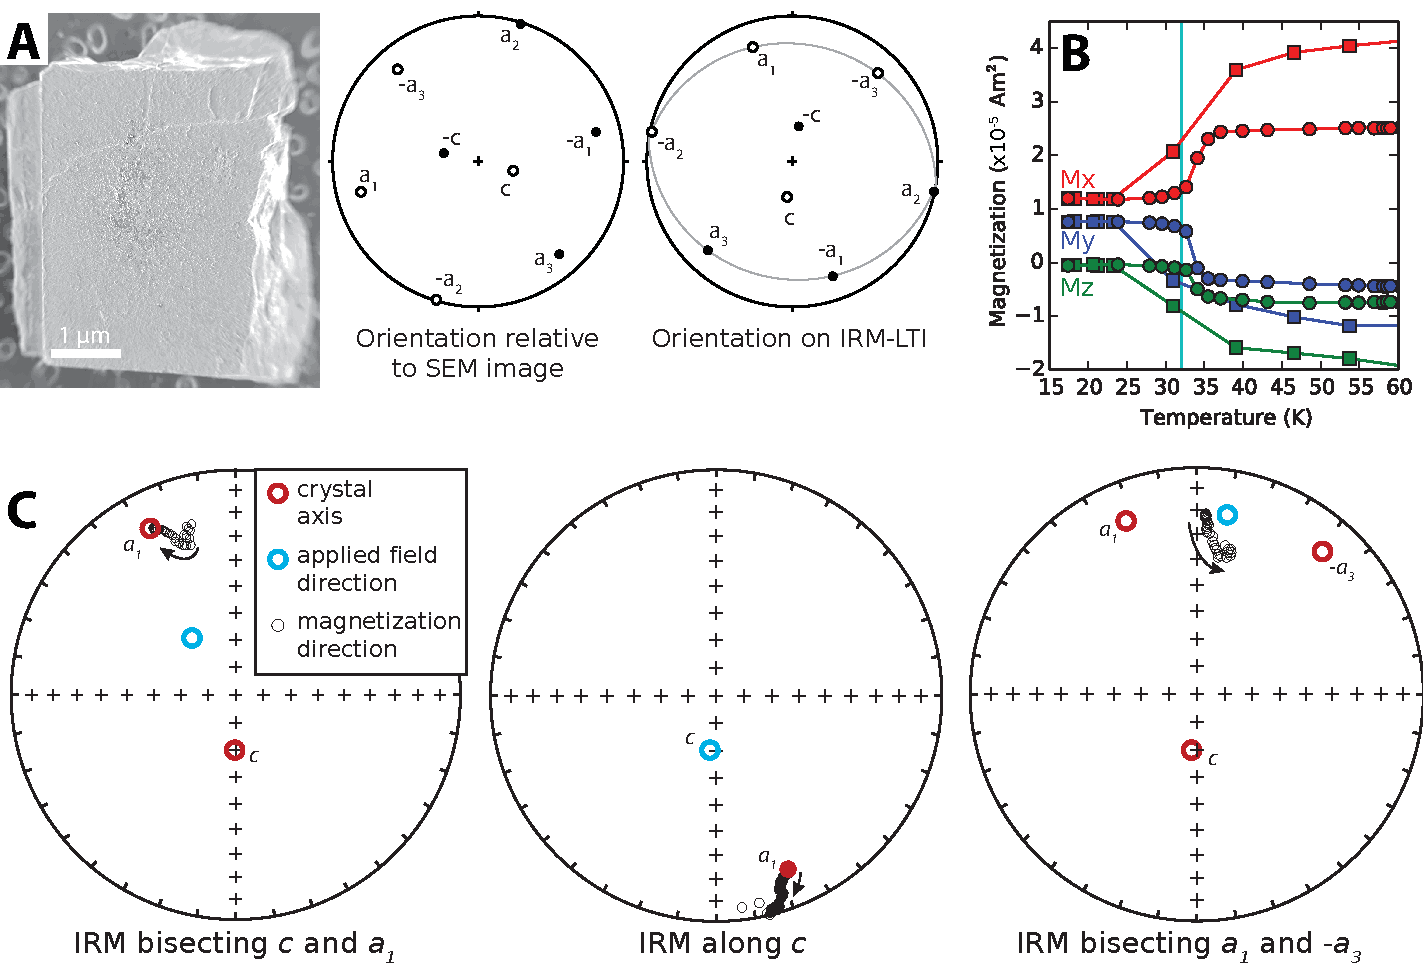
\includegraphics[width=\textwidth]{Pyrrhotite1.pdf}
\caption{Experiments conducted on a single crystal of pyrrhotite. (a) Secondary electron SEM micrograph of the sample and crystal orientation information during the progression of an experiment. (b) three-axis low-temperature remanence data upon cooling (squares) and warming (circles) for the IRM bisecting c and a$_1$ experiment. The Besnus transition is well-expressed in these data and closely corresponds with the canonical value for the transition (32 K) shown with the cyan vertical line. (c) Equal area plots showing the directional data (black circles with arrow indicating direction of change) obtained upon cooling for isothermal remanent magnetizations (IRM) that were applied in three different directions. The direction along which the 1.2 T pulse magnetizations were applied are indicated in each plot with a light blue circle, relevant crystal axis directions are shown with red circles while the data during the low-temperature cycling are shown with small grey circles.}
\label{fig:pyrrhotite}
\end{figure}

\begin{figure}
\noindent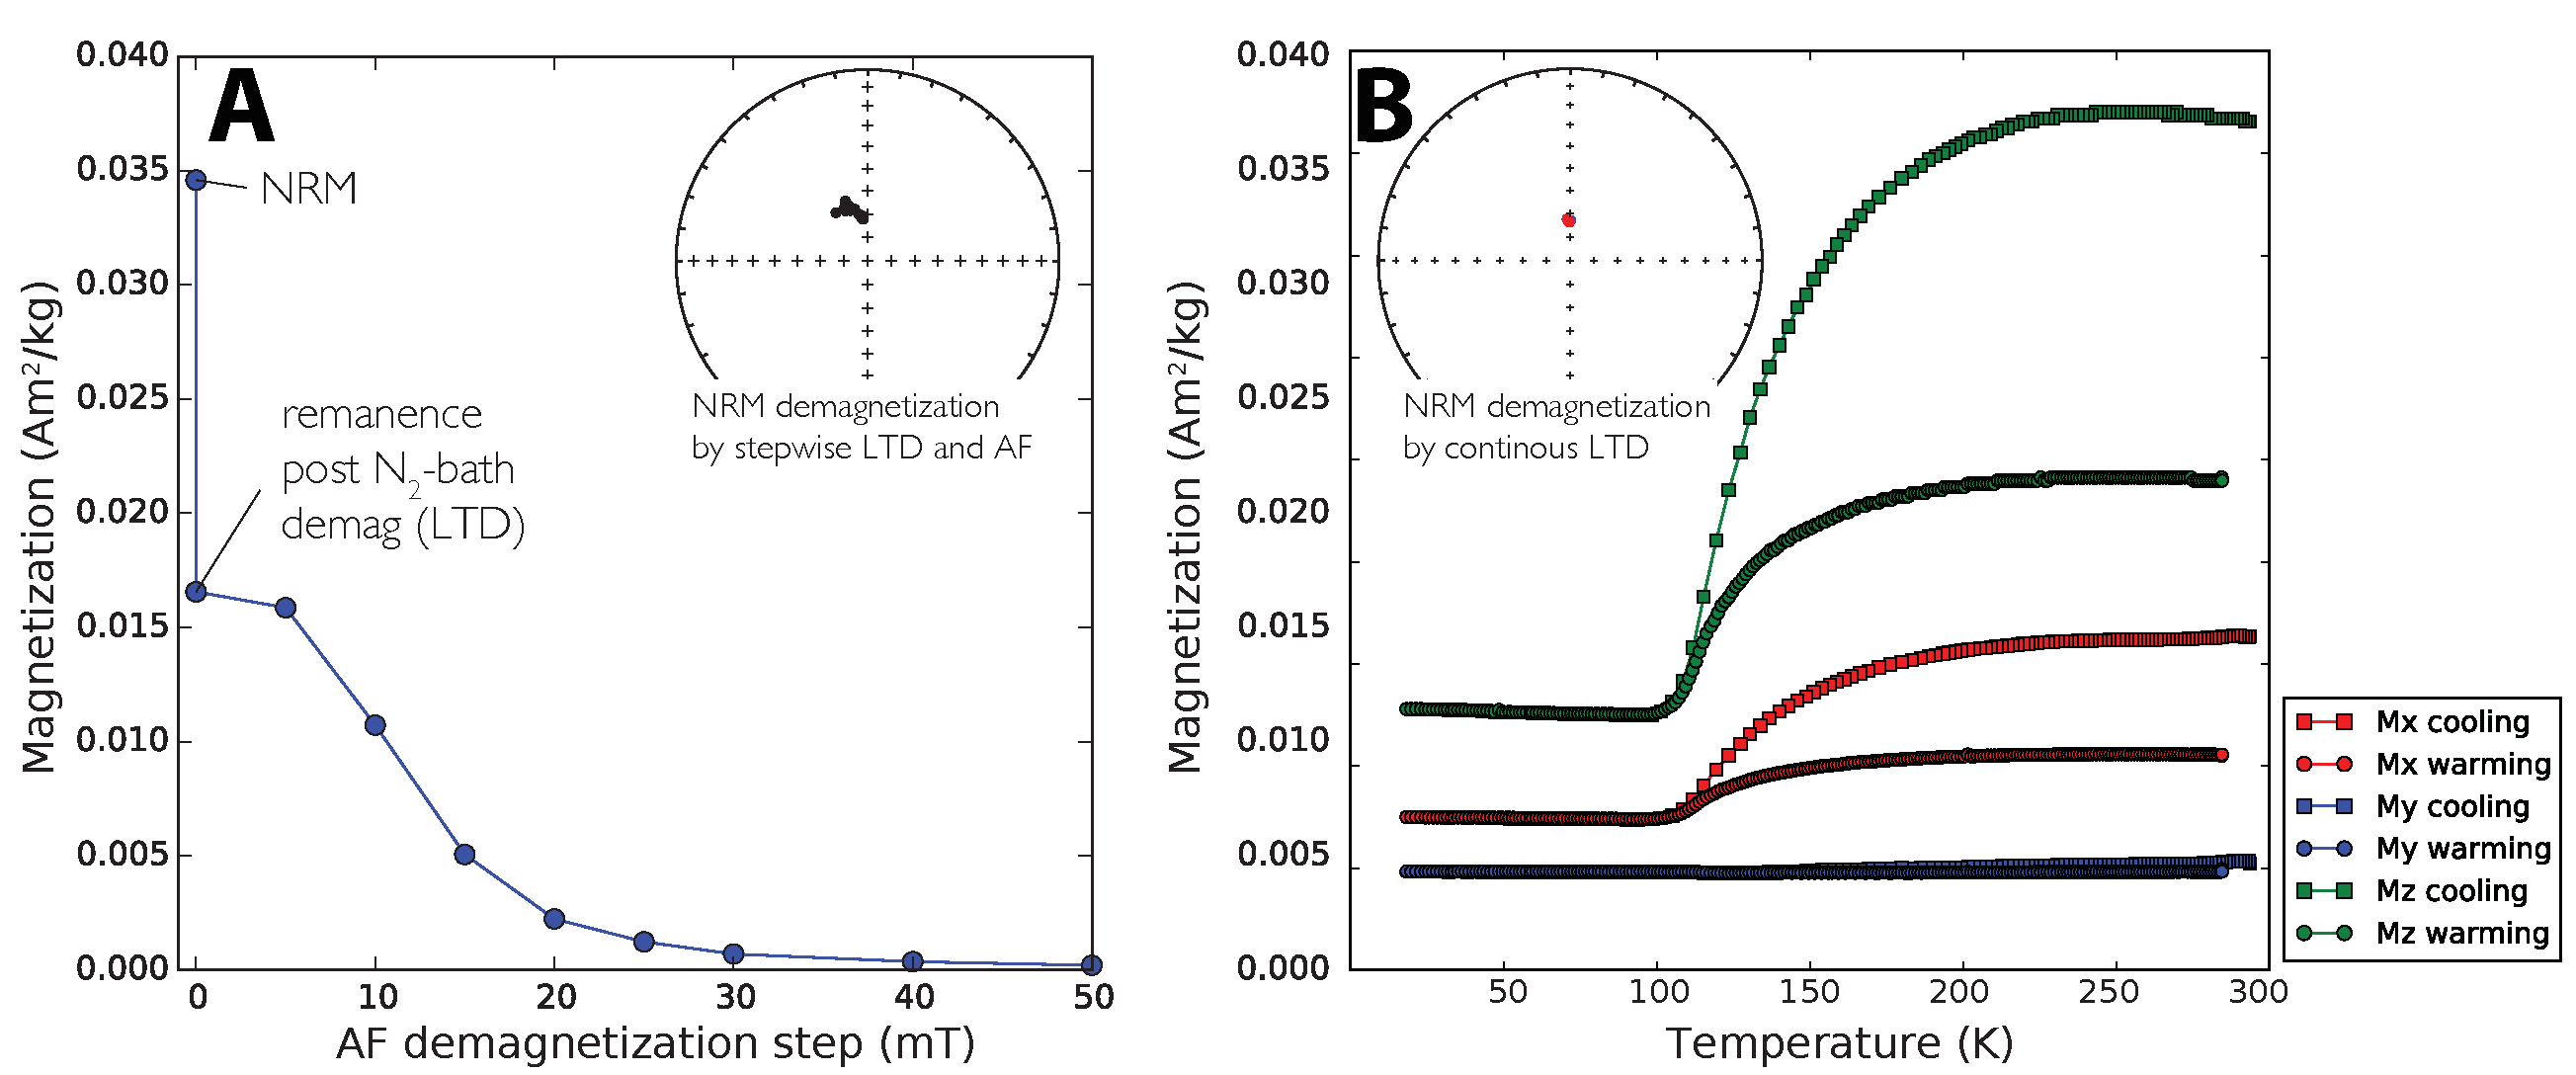
\includegraphics[width=\textwidth]{Umkondo_PW15_NRM.pdf}
\caption{Natural remanent magnetization (NRM) data for a coarse-grained diabase sill sample (PW15-4a). (a) Demagnetization data that begins with a low-temperature demagnetization step (a liquid N$_2$ bath in near zero field) followed by AF demagnetization. The remanence is comprised of a single directional component as can be seen in the inset equal area plot. (b) Three-axis low-temperature cycling data of NRM obtained on the IRM-LTI for the natural remanence of a sister specimen from the same sample. The directions are summarized on the inset equal area plot and are very similar to the directions of the step-wise AF demagnetization data.}
\label{fig:Umkondo_PW15NRM}
\end{figure}

\begin{figure}
\noindent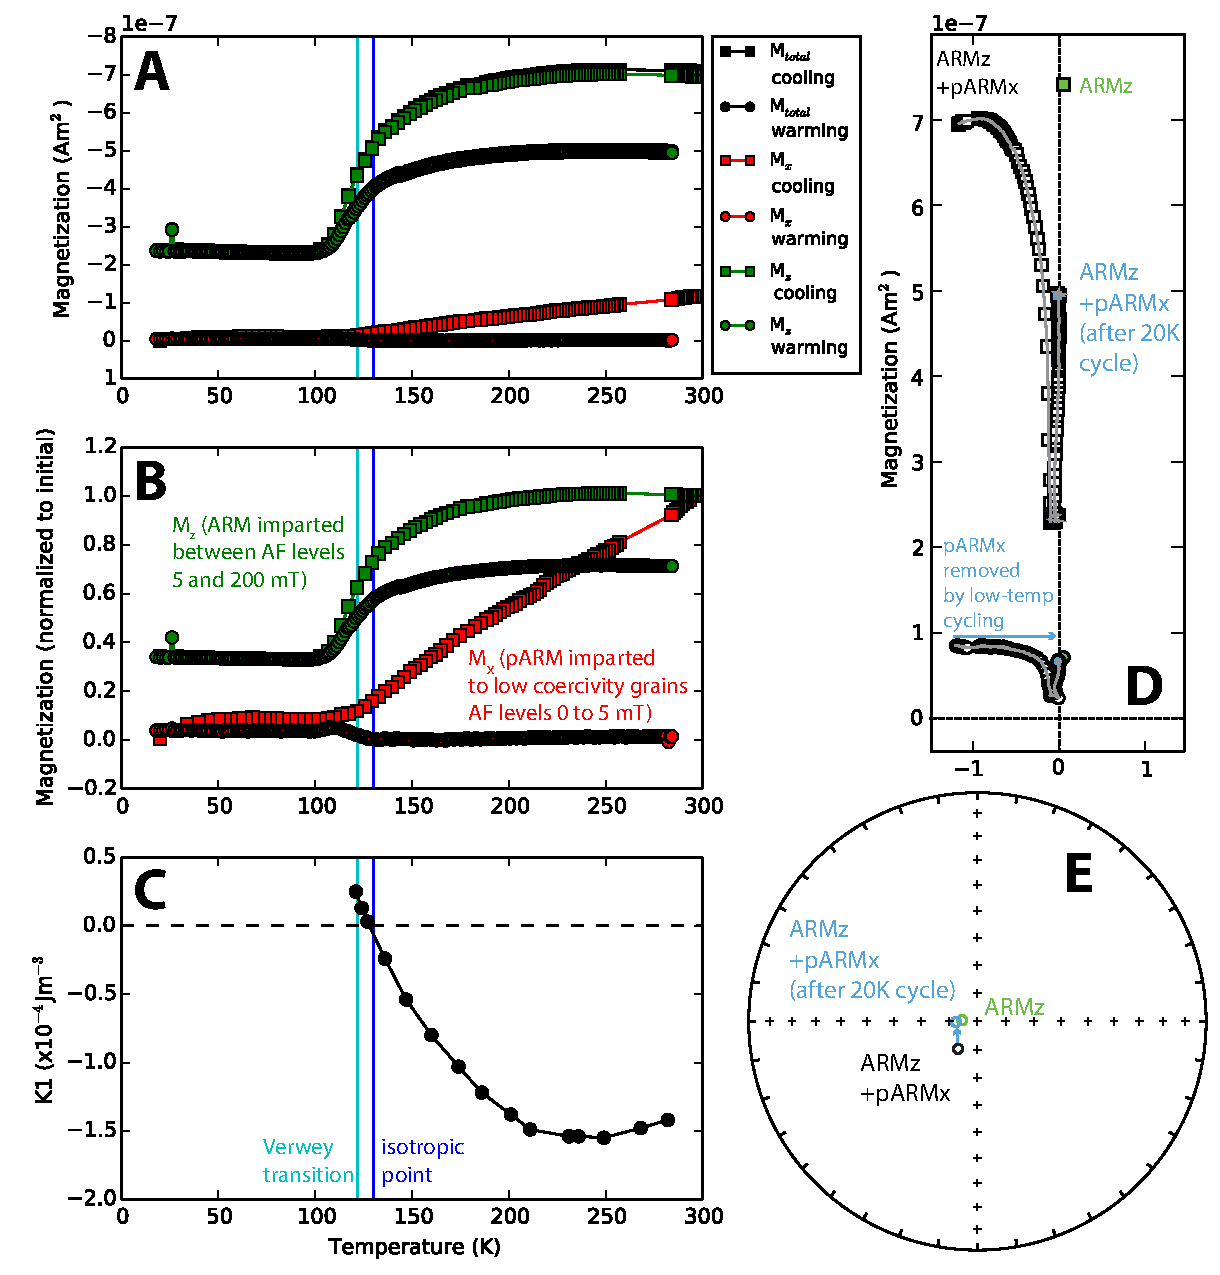
\includegraphics[width=0.8\textwidth]{PW15-4d_ARMex.pdf}
\caption{Low-temperature behavior of an ARM applied to the z-axis and a pARM applied to the x-axis of a specimen of an Umkondo diabase sill (PW15-4d). (a) shows the magnetization of the z and x components as well as the total magnetization upon cooling (note that the y-axis of the plot is inverted for comparison between the components and the total magnetization). The z and x components are normalized to their initial magnetizations in (b) to highlight the differing behavior between the x-axis magnetization (pARM imparted to low coercivity grains) and the z-axis magnetization (ARM on the rest of the coercivity spectrum). (c) shows the magnetocrystalline anisotropy constant K$_1$ as a function of temperature (data of \cite{Bickford1957a} as presented in \cite{Muxworthy2000b}). The vector-component diagram (d) and equal area plot (e) show the directional change associated with low-temperature cycling and illustrate the return to the direction of the z-axis ARM with the x-axis pARM demagnetized.}
\label{fig:Umkondo_ARM}
\end{figure}

\begin{figure}
\noindent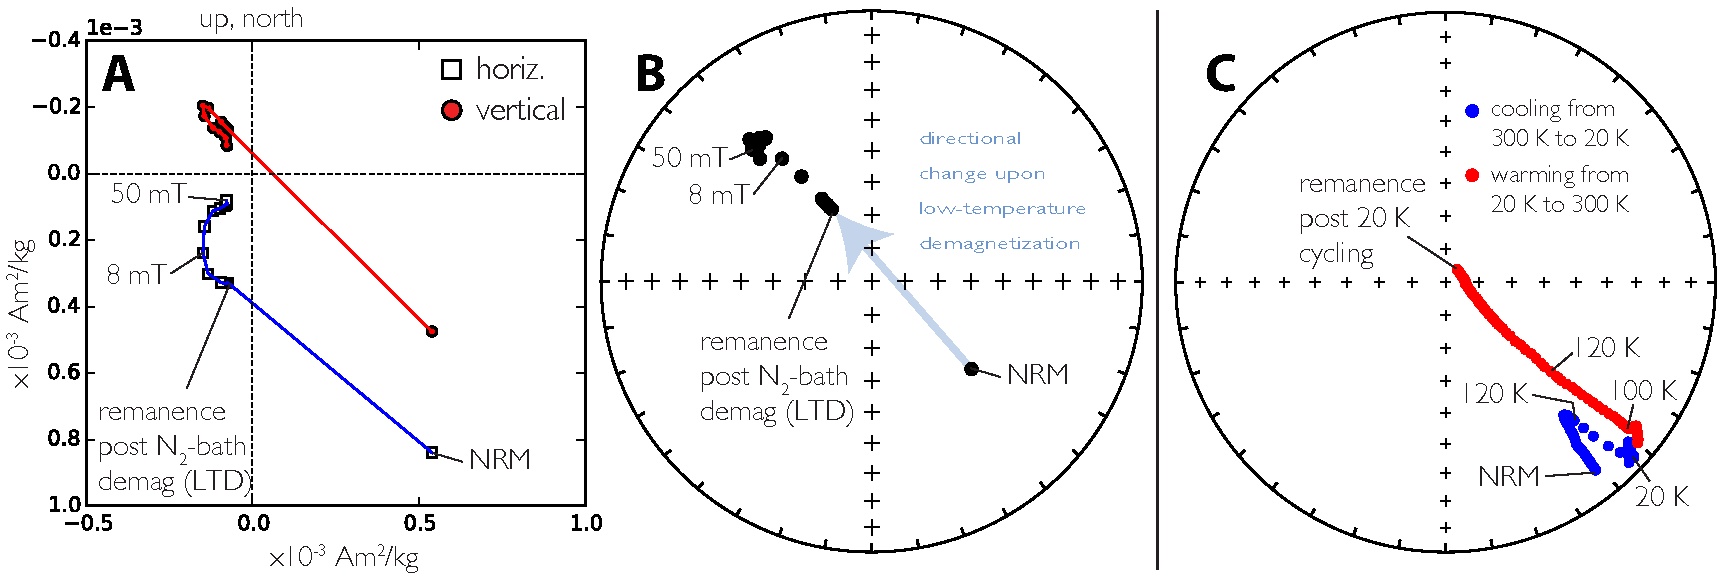
\includegraphics[width=\textwidth]{Umkondo_PW10_NRM.pdf}
\caption{Natural remanent magnetization (NRM) data for a coarse-grained diabase sill sample (PW10-7). (a) Demagnetization data that begins with a low-temperature demagnetization step (a liquid N$_2$ bath) followed by AF demagnetization. The vector component diagram in (a) and equal area plot in (b) show significant loss of remanence and directional change that accompanied the liquid N$_2$ treatment. (c) Low-temperature cycling of the NRM of a sister specimen on the IRM-LTI documented  directional change throughout the experiment with movement in the direction of overprint removal both during cooling  to the Verwey transition and upon warming back across the Verwey transition.}
\label{fig:Umkondo_PW10NRM}
\end{figure}

\end{document}
